162. \begin{figure}[ht!]
\center{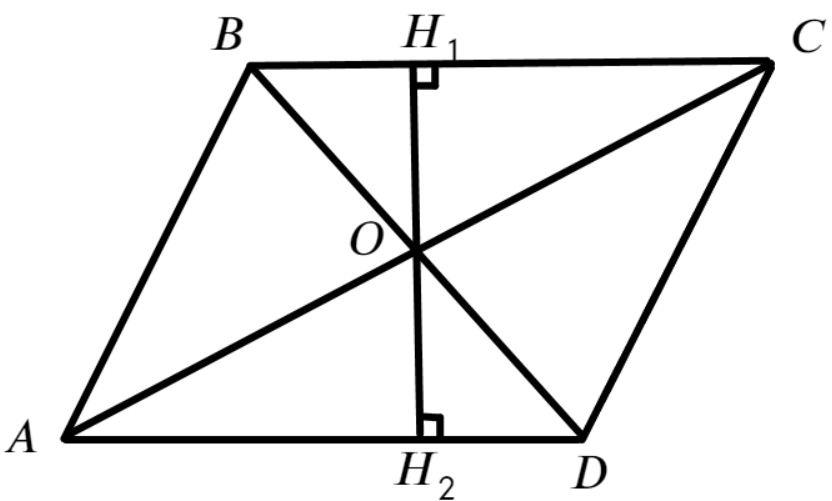
\includegraphics[scale=0.35]{g9-161.png}}
\end{figure}\\
Так как в параллелограмме диагонали делятся точкой пересечения пополам, имеем равенства $AO=OC,\ DO=OB.$ Также $BC=AD$ как противоположные стороны параллелограмма, а значит треугольники $AOD$ и $BOC$ равны по трём сторонам, поэтому в них равны соответствующие высоты и $H_1H_2=OH_1+OH_2=3+3=6$см. Тогда $S_{ABCD}=H_1H_2\cdot AD=6\cdot14=84\text{ см}^2.$
